% ============================================================================
% Hexera CAD Repair System - customer white paper
%
% This is the SALES document. Audience: an engineering lead evaluating CRS.
% main.tex is the technical paper; full-paper.tex is the long form. Those two
% carry the method, the controls and the limits.
%
% It deliberately shares main.tex's preamble, title block, heading scheme,
% figure and table style, so the two read as one family of documents.
%
% RULES FOR THIS FILE, so it stays sellable AND survives first contact:
%   - Every number here is measured and traceable to a committed evidence
%     bundle. Do not round up, do not extrapolate, do not add a figure that
%     exists only in a deck.
%   - Only describe capability that is on by default or demonstrable on
%     request. Nothing here should promise work that is still behind a flag.
%   - Omitting internal detail is fine. Implying a capability we cannot show
%     on the customer's own parts is not: they will run it within the week.
%
% Overleaf: compiler pdfLaTeX, main document customer-brief.tex.
% Locally: latexmk -pdf customer-brief.tex
% ============================================================================
\documentclass[10pt,onecolumn]{article}

\usepackage[T1]{fontenc}
\usepackage{charter}
\usepackage[scaled=0.84]{beramono}
\usepackage[letterpaper,margin=0.95in]{geometry}
\usepackage{microtype}
\setlength{\emergencystretch}{1.2em}
\usepackage{booktabs}
\usepackage{tabularx}
\usepackage{array}
\usepackage{tikz}
\usetikzlibrary{arrows.meta,positioning,calc}
\usepackage[labelfont=bf,font=small,skip=5pt]{caption}
\usepackage{enumitem}
\usepackage{titlesec}
\usepackage{fancyhdr}
\usepackage[hidelinks]{hyperref}

% ---- paragraph style: block, not indented, applied everywhere -------------
\setlength{\parindent}{0pt}
\setlength{\parskip}{0.62\baselineskip}

% ---- headings --------------------------------------------------------------
\titleformat{\section}{\normalfont\large\bfseries}{\thesection}{0.7em}{}
\titleformat{\subsection}{\normalfont\normalsize\bfseries}{\thesubsection}{0.7em}{}
\titlespacing*{\section}{0pt}{1.15\baselineskip}{0.35\baselineskip}
\titlespacing*{\subsection}{0pt}{0.85\baselineskip}{0.25\baselineskip}
\newcommand{\topic}[1]{\textbf{#1.}\hspace{0.5em}\ignorespaces}

% ---- lists: hang from the text block, even spacing -------------------------
\setlist{nosep}
\setlist[itemize]{leftmargin=1.5em,labelindent=0pt,labelwidth=0.8em,labelsep=0.7em,
                  align=left,label=\textbullet,itemsep=5pt,topsep=5pt}
\setlist[enumerate]{leftmargin=2.1em,labelindent=0pt,labelwidth=1.4em,labelsep=0.7em,
                    align=left,label=\arabic*.,itemsep=5pt,topsep=5pt}

\pagestyle{fancy}
\fancyhf{}
\renewcommand{\headrulewidth}{0.4pt}
\fancyhead[C]{\footnotesize\itshape Hexera CAD Repair System --- White Paper}
\fancyfoot[C]{\thepage}
\fancypagestyle{plain}{\fancyhf{}\renewcommand{\headrulewidth}{0pt}\fancyfoot[C]{\thepage}}

\newcommand{\code}[1]{\texttt{\small #1}}
\newcolumntype{L}[1]{>{\raggedright\arraybackslash}p{#1}}

\tikzset{
  blk/.style={draw,thin,rectangle,align=center,inner sep=2.5pt,font=\scriptsize,
              minimum height=8.5mm,text width=21mm},
  sblk/.style={blk,text width=17mm,minimum height=5.5mm},
  ar/.style={-{Latex[length=1.5mm,width=1.1mm]},thin},
  lbl/.style={font=\scriptsize\itshape,text=black!60},
}

\title{\vspace{-1.3cm}\bfseries Repairing Imported CAD Before It Blocks Your Mesh\\[0.2em]
       \large\normalfont\itshape The Hexera CAD Repair System: what it repairs, what it guarantees
       and what it measures}
\author{Hexera}
\date{White Paper, Revision 2 --- November 2026}

\begin{document}
\maketitle
\thispagestyle{plain}

\begin{abstract}
\noindent
Simulation schedules are set less often by solver time than by geometry. A supplier's STEP file
arrives with shells that no longer close and features smaller than any element the analysis
intends to mesh; the mesher refuses it, and an engineer spends an afternoon repairing it in a CAD
tool, then repeats that work at the next revision. The Hexera CAD Repair System (CRS) is designed
to remove that step from the critical path. It locates every defect in an incoming part, repairs
what it can with bounded CAD-kernel operations, and measures the result against the uploaded file
before releasing anything; repairs that do not improve the part are rolled back, and the uploaded
file is never modified. Parts it cannot repair are returned with the responsible geometry named
and located. This paper describes what CRS repairs, the limits every repair is held inside, what
is returned with the geometry, and results measured on public parts that can be downloaded and
re-run: 430 defects repaired across a 331-file dataset, a race-car body taken from invalid to
valid with all eight bodies intact and mesh-engine staging time halved, and 40 clean reference
parts returned unchanged.
\end{abstract}

% =============================================================== 1 ==========
\section{The Problem}

Geometry for analysis usually originates elsewhere: with a supplier, or with another team on
another CAD system, and it is exchanged as STEP. That round trip is lossy. Faces arrive without
the edges they shared, so shells that were closed are now open. Trimming curves drift from the
surfaces they bound. Edges a few microns long survive the export into a model that will be meshed
in millimetres. Some of this breaks the CAD kernel's validity rules; much of it is valid and still
will not mesh. In either case the mesher rejects the part before a boundary condition has been
set.

The repair is then done by hand in a CAD tool. It occupies an experienced engineer for an
afternoon, and the work recurs when the supplier issues a revision. Across several suppliers and
several revisions each, this is a material constraint on how many studies a team completes, and it
is one reason batch simulation remains difficult: a pipeline that stalls on a single unmeshable
part requires someone to be watching it.

% =============================================================== 2 ==========
\section{How CRS Works}\label{sec:how}

CRS sits between CAD intake and meshing, ahead of whichever mesh engine is already in use
(Figure~\ref{fig:pipeline}). It inspects the incoming part, pins each defect to the entity
carrying it, and repairs what it can with bounded CAD-kernel operations. Before anything is
released it measures the result against the original file and stages it for the mesher. A part
that passes is ready to mesh at the end of that inspection, without waiting on an engineer.

\begin{figure}[h]
\centering
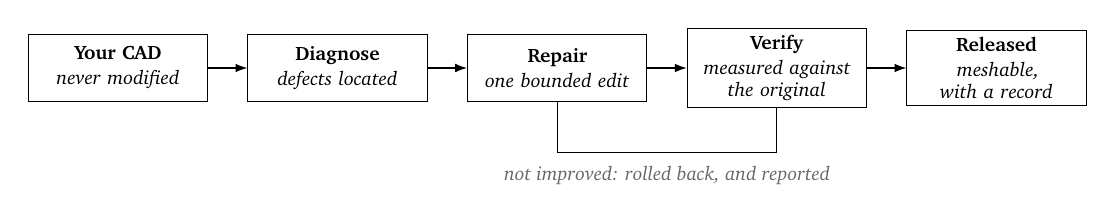
\begin{tikzpicture}[node distance=5mm]
  \node[blk] (up)  {\textbf{Your CAD}\\[1pt]\scriptsize\itshape never modified};
  \node[blk,right=of up]  (ins) {\textbf{Diagnose}\\[1pt]\scriptsize\itshape defects located};
  \node[blk,right=of ins] (rep) {\textbf{Repair}\\[1pt]\scriptsize\itshape one bounded edit};
  \node[blk,right=of rep] (ver) {\textbf{Verify}\\[1pt]\scriptsize\itshape measured against the original};
  \node[blk,right=of ver] (out) {\textbf{Released}\\[1pt]\scriptsize\itshape meshable, with a record};
  \foreach \a/\b in {up/ins,ins/rep,rep/ver,ver/out} \draw[ar] (\a) -- (\b);
  \coordinate (lo) at ($(rep.south)!0.5!(ver.south)+(0,-6mm)$);
  \draw[thin] (ver.south) -- (ver|-lo) -- (rep|-lo) -- (rep.south);
  \node[lbl,below=0.5mm of lo] {not improved: rolled back, and reported};
\end{tikzpicture}
\caption{Repair as a measured, reversible step. Each edit is checked against the uploaded part
before it is allowed to stand, so geometry that cannot be improved is reported rather than
altered.}
\label{fig:pipeline}
\end{figure}

\subsection{Guarantees}

\topic{Your upload is never touched} Repairs are written to a separate artefact. The file you sent
remains byte-for-byte the file you sent, and the repaired part is delivered alongside it.

\topic{Nothing is released that was not verified} Every candidate repair is measured against your
original: kernel validity, solid count, face count, surface area, volume, tolerance and the
distance any surface moved. A candidate that fails any one of these is rolled back, and the part is
reported as needing attention rather than quietly altered.

\topic{It leaves your design alone} No feature is deleted to force a part through the mesher. An
opening whose rim pairs with another is recognised as a through-passage and left open, because
patching both ends would seal a passage somebody drew deliberately. Every repair is held inside
conservative geometric limits, and those limits are checked against the file you sent rather than
against the previous edit, so a sequence of small repairs stays faithful to the part you
uploaded.

\topic{Every run leaves a record} You get the list of what was wrong and where it sat. Against each
entry: what CRS did about it, the measurements either side of the edit, and where it did nothing,
the reason. When somebody in a design review asks why a face moved, the answer is in the file
rather than in an engineer's memory of a Tuesday afternoon.

% =============================================================== 3 ==========
\section{What CRS Repairs}

Table~\ref{tab:coverage} lists the geometry problems CRS detects and addresses. The vocabulary is
deliberately narrow and stable, because a defect report is only useful if the same problem is
called the same thing on every part, every run.

\begin{table}[h]
\centering
\caption{Geometry problems CRS finds and repairs, with the kernel operation behind each. Detection
always runs; which repairs are enabled is a deployment decision, set once rather than per part.}
\label{tab:coverage}
\footnotesize
\begin{tabularx}{\textwidth}{@{}L{46mm} X@{}}
\toprule
\textbf{Problem in your geometry} & \textbf{What CRS does about it}\\
\midrule
Open shells and free boundaries
  & Sews the boundaries back together so the surfaces close into the solid the mesher is waiting
    for.\\
Missing faces and bounded openings
  & Patches an isolated opening, flat or curved, up to a strict size. Anything bigger reads as a
    missing wall and is refused.\\
Edges and faces below mesh scale
  & Takes out slivers and near-zero edges. These are what force a mesher into elements no solver
    wants to see.\\
Broken face boundaries
  & Repairs wire ordering and the parameter-space curves that stop agreeing with their surfaces
    after translation.\\
Self-intersecting wires and faces
  & Heals crossings the CAD kernel can identify and locate on the part.\\
Invalid B-rep topology
  & A bounded global pass, used only when the local repairs have left the part invalid.\\
Closed, periodic surfaces
  & Splits a full cylinder or sphere at its seam. A surprising number of refusals come down to
    this.\\
Bodies in contact in an assembly
  & Gives two touching bodies a shared interface the volume mesher can work with. Both bodies stay
    separate parts.\\
Faces the surface mesher cannot resolve
  & Re-trims the single offending face from its own boundary, leaving the underlying surface
    unchanged.\\
\bottomrule
\end{tabularx}
\end{table}

Detection does not depend on repair being switched on. Run CRS with every repair disabled and it
still sorts your parts into the sound and the broken, and points at the geometry responsible. Some
teams start there deliberately, and turn repairs on once they have seen a few hundred parts
triaged.

% =============================================================== 4 ==========
\section{What Comes Back}

Every part leaves CRS carrying a disposition, and that disposition is part of the result rather
than a line in a log. A part with no blocking defect, or whose only findings are ones your workflow
already accepts, comes back ready to mesh. A part whose blocking defects were fixed within every
limit, and which then staged successfully for the mesh engine, comes back repaired, as a new
artefact alongside the original. Where the geometry is understood but the right change depends on
design intent, the part is routed to an engineer with its findings and their locations attached, so
the work starts from a diagnosis rather than a blank part and a complaint from the mesher. The
remaining case is a part that raises a question only its author can answer, which comes back to you
with that question stated.

Alongside the geometry you get the record: every defect with its location, the operation applied to
it, the measurements taken before and after, and the reason for anything left untouched. That
record is produced on every run rather than enabled specially, and because repaired artefacts are
content-addressed, sending the same part through again returns byte-identical output. A result can
be regenerated and compared months later, which is what makes repaired geometry usable in a
qualification package. CRS runs as a step ahead of whichever mesh engine is already in use, and is
configured once per deployment rather than per part. Where a deployment turns it on, verification
goes one step further and meshes the repaired part for real, so the question answered is whether
the part meshes rather than whether a kernel is satisfied with it. That is the strictest setting
CRS has, and it is the one we normally run during an evaluation.

% =============================================================== 5 ==========
\section{Measured Results}\label{sec:results-anchor}

The figures below come from public, reproducible geometry rather than internal fixtures, so they
can be checked independently.

\subsection{At corpus scale}

Against the 331-file public OpenCASCADE test dataset, CRS repairs \textbf{430 defects} in a single
run, the bulk of them open shells and sub-scale edges. Every file it releases as repaired passes an
independent final re-inspection and stages successfully for the mesh engine.

Just as important is what happens to the rest of the dataset, because a repair tool is judged on
the parts it cannot fix as much as the ones it can. Of the remaining files, 143 are reported as
needing nothing, 115 are refused with the reason recorded, and 57 are routed to a person as
questions of design intent. Nothing is passed through unexamined, and nothing is altered on a
guess.

\subsection{On a full vehicle body}

A public Formula 1000 race-car body, used exactly as received, fails the OpenCASCADE validity
check. After CRS it passes, with all eight solid bodies intact and the part's overall dimensions
unchanged (Table~\ref{tab:f1000}). The repaired body also reached the mesh engine in under half the
time.

The result is conservative by design. The initial inspection found 171 issues on this body; CRS
cleared the ones blocking the mesh and left 162 warning-level findings in place, because removing
them would mean defeaturing a vehicle body whose small features may carry the aerodynamics. On the
companion front-suspension rocker from the same model, findings fell from 12 to 8 and sliver faces
from four to one, with the single solid body preserved and the part still valid.

\begin{table}[h]
\centering
\caption{Formula 1000 race-car body, before and after CRS. Public model, used as received; figures
from a single run.}
\label{tab:f1000}
\footnotesize
\begin{tabularx}{\textwidth}{@{}l r r >{\raggedright\arraybackslash}X@{}}
\toprule
\textbf{Measure} & \textbf{Before} & \textbf{After} & \textbf{What it means for you}\\
\midrule
CAD kernel validity & invalid  & \textbf{valid}   & The blocking error is gone; the part is usable downstream.\\
Solid bodies        & 8        & 8                & Nothing lost, nothing merged.\\
Faces               & 421      & 419              & Bounded clean-up only; extents unchanged.\\
Mesh engine staging & 16.87\,s & \textbf{7.99\,s} & The repaired part reached the mesher in under half the time.\\
\bottomrule
\end{tabularx}
\end{table}

\subsection{Cost of a run}

CRS proves each repair locally instead of re-checking the whole part after every edit. On a 50-part
benchmark this cuts the expensive whole-part inspections from \textbf{566 to 54}, with the worst
single part falling from 45 to 2, and total runtime falling as well (Table~\ref{tab:cost}). Across
those 50 parts, \textbf{41 improved, 9 were unchanged, and none came out worse.}

In absolute terms the whole 50-part set completes in 154 seconds, so verification costs tens of
seconds per part. That is the figure to compare against the time the same parts take to repair by
hand, and it is what makes the step viable inside an automated pipeline rather than only as an
interactive tool.


\subsection{Safe on parts that need no repair}

Run against 40 clean reference parts spanning 22 part families, CRS made \textbf{no changes at
all}: no operation kept, and no face, solid or volume altered. A tool that edits geometry which was
never broken is a liability in a simulation pipeline, so this is tested directly on every release
rather than assumed.

\begin{table}[h]
\centering
\caption{Cost of repair on a 50-part benchmark, and behaviour on 40 clean reference parts drawn
across 22 part families.}
\label{tab:cost}
\footnotesize
\begin{tabularx}{\textwidth}{@{}X r r@{}}
\toprule
 & \textbf{Conventional} & \textbf{CRS}\\
\midrule
Whole-part inspections, 50-part benchmark & 566    & \textbf{54}\\
Worst case on a single part               & 45     & \textbf{2}\\
Total runtime                             & 184\,s & \textbf{154\,s}\\
Per-part outcome                          & ---    & \textbf{41 improved, 9 tied, 0 worse}\\
Clean parts: edits kept / parts changed   & ---    & \textbf{0 / 0}\\
\bottomrule
\end{tabularx}
\end{table}

% =============================================================== 6 ==========
\section{Mesh-Aware Verification}

Kernel validity and meshability are not the same property, and a part can satisfy the first while
failing the second. CRS can therefore mesh the part itself as part of verification rather than
reasoning only about the B-rep.

The probe runs gmsh on the shape in an isolated child process, with element size set from the
bounding-box diagonal and a bounded time budget, and treats a part as meshable when it yields
volume elements. Two things follow from that. A repair aimed at a meshing failure is judged on
whether the part meshes afterwards, not merely on whether the kernel is satisfied. And when a mesh
fails, the failing surface tag is mapped back through the shape's own face map to a face
fingerprint, so the failure is reported against the geometry carrying it: a named face for a
surface-stage failure, or the pair of bodies in contact for an assembly that fails in the volume
stage. A failure that cannot be tied to an entity is reported as unlocated rather than attributed
to a guess.

This matters most for the families where the mesher's own diagnostics are least useful --- contact
between bodies in an assembly, overlapping facets on a trimmed face, a closed cylindrical surface
carrying a single seam. In each case the mesher reports a symptom in its own coordinates, and the
work of finding the responsible geometry is the slow part of the job.

% =============================================================== 7 ==========
\section{In Development}

One rule governs this section: nothing described here is part of what an evaluation runs today, and
nothing in it should be read as a capability. We describe the direction because engineers evaluating
CRS reasonably ask where it is going, and because a claim made early is a claim we would have to
withdraw.

\topic{Repair as a job in its own right} CRS was built as the stage before meshing. It is being
generalised so that clean CAD is a deliverable on its own, with the same limits, the same rollback
and the same per-part record, for teams whose problem is the geometry rather than the mesh.

\topic{A deeper look at the hard parts} The families that resist repair today are the ones where the
right answer depends on engineering judgement: whether two bodies in an assembly are meant to share
an interface, or whether a fault lies in the CAD or in the mesher. We are extending the system so
that a difficult region is investigated --- measured, probed, and edited on a throwaway copy ---
before any change is proposed against the real part, and so that several candidate repairs can be
rehearsed on copies and only the best one offered for review. The guarantees in
Section~\ref{sec:how} are unchanged by this work and are what bound it: every candidate is still
measured against your uploaded file, still rolled back unless it improves the part, and still
reviewed before anything is released.

\topic{What we will not do with it} We report a gain from this work only as it is measured on real
failing parts, scored against the deterministic baseline it has to beat, with the number of parts it
broke reported beside the number it fixed. Section~\ref{sec:v3brief} holds that measurement. The
figures in Section~\ref{sec:results-anchor} are measured on the deterministic system you would be
evaluating.

% ============================================================ v3 results ====
% The values below are generated from sealed evidence by
% devtools/validation/v3_eval/results_to_tex.py. A [PENDING] value has not been measured. Under this
% brief's rule, do not send a customer a copy that still prints [PENDING]: either the runs have
% landed and the numbers stand, or this section is cut from the copy that goes out.
\section{Measured Results (CRS v3)}\label{sec:v3brief}

% GENERATED by devtools/validation/v3_eval/results_to_tex.py - do not edit by hand.
% source: devtools/validation/v3_eval/results.pending.json
% generated_at: unknown
% A [PENDING] value has not been measured. It is never a zero.
% \providecommand so the file can be \input more than once and override nothing.
\providecommand{\vThreeRulesOnlyNFiles}{\textbf{[PENDING]}}
\providecommand{\vThreeRulesOnlyNewlyMeshed}{\textbf{[PENDING]}}
\providecommand{\vThreeRulesOnlyNewlyBroken}{\textbf{[PENDING]}}
\providecommand{\vThreeRulesOnlyMeshesBefore}{\textbf{[PENDING]}}
\providecommand{\vThreeRulesOnlyMeshesAfter}{\textbf{[PENDING]}}
\providecommand{\vThreeRulesOnlyModelCalls}{\textbf{[PENDING]}}
\providecommand{\vThreeRulesOnlyCostUsd}{\textbf{[PENDING]}}
\providecommand{\vThreeRulesOnlyWallS}{\textbf{[PENDING]}}
\providecommand{\vThreeRulesOnlyCostPerFixed}{\textbf{[PENDING]}}
\providecommand{\vThreeRulesOnlyCommit}{\textbf{[PENDING]}}
\providecommand{\vThreeRulesOnlyImage}{\textbf{[PENDING]}}
\providecommand{\vThreeRulesOnlySample}{\textbf{[PENDING]}}
\providecommand{\vThreeRulesOnlyEndings}{\textbf{[PENDING]}}
\providecommand{\vThreeRulesOnlyOpsKept}{\textbf{[PENDING]}}
\providecommand{\vThreeRulesOnlyOpsRolledBack}{\textbf{[PENDING]}}
\providecommand{\vThreeRulesOnlyLabel}{rules-only baseline}
\providecommand{\vThreeDetNFiles}{\textbf{[PENDING]}}
\providecommand{\vThreeDetNewlyMeshed}{\textbf{[PENDING]}}
\providecommand{\vThreeDetNewlyBroken}{\textbf{[PENDING]}}
\providecommand{\vThreeDetMeshesBefore}{\textbf{[PENDING]}}
\providecommand{\vThreeDetMeshesAfter}{\textbf{[PENDING]}}
\providecommand{\vThreeDetModelCalls}{\textbf{[PENDING]}}
\providecommand{\vThreeDetCostUsd}{\textbf{[PENDING]}}
\providecommand{\vThreeDetWallS}{\textbf{[PENDING]}}
\providecommand{\vThreeDetCostPerFixed}{\textbf{[PENDING]}}
\providecommand{\vThreeDetCommit}{\textbf{[PENDING]}}
\providecommand{\vThreeDetImage}{\textbf{[PENDING]}}
\providecommand{\vThreeDetSample}{\textbf{[PENDING]}}
\providecommand{\vThreeDetEndings}{\textbf{[PENDING]}}
\providecommand{\vThreeDetOpsKept}{\textbf{[PENDING]}}
\providecommand{\vThreeDetOpsRolledBack}{\textbf{[PENDING]}}
\providecommand{\vThreeDetLabel}{deterministic catalogue (investigator and tournament off)}
\providecommand{\vThreeNFiles}{\textbf{[PENDING]}}
\providecommand{\vThreeNewlyMeshed}{\textbf{[PENDING]}}
\providecommand{\vThreeNewlyBroken}{\textbf{[PENDING]}}
\providecommand{\vThreeMeshesBefore}{\textbf{[PENDING]}}
\providecommand{\vThreeMeshesAfter}{\textbf{[PENDING]}}
\providecommand{\vThreeModelCalls}{\textbf{[PENDING]}}
\providecommand{\vThreeCostUsd}{\textbf{[PENDING]}}
\providecommand{\vThreeWallS}{\textbf{[PENDING]}}
\providecommand{\vThreeCostPerFixed}{\textbf{[PENDING]}}
\providecommand{\vThreeCommit}{\textbf{[PENDING]}}
\providecommand{\vThreeImage}{\textbf{[PENDING]}}
\providecommand{\vThreeSample}{\textbf{[PENDING]}}
\providecommand{\vThreeEndings}{\textbf{[PENDING]}}
\providecommand{\vThreeOpsKept}{\textbf{[PENDING]}}
\providecommand{\vThreeOpsRolledBack}{\textbf{[PENDING]}}
\providecommand{\vThreeLabel}{CRS v3 (investigator live, tournament live, K=3)}
\providecommand{\vThreeTourOffNFiles}{\textbf{[PENDING]}}
\providecommand{\vThreeTourOffNewlyMeshed}{\textbf{[PENDING]}}
\providecommand{\vThreeTourOffNewlyBroken}{\textbf{[PENDING]}}
\providecommand{\vThreeTourOffMeshesBefore}{\textbf{[PENDING]}}
\providecommand{\vThreeTourOffMeshesAfter}{\textbf{[PENDING]}}
\providecommand{\vThreeTourOffModelCalls}{\textbf{[PENDING]}}
\providecommand{\vThreeTourOffCostUsd}{\textbf{[PENDING]}}
\providecommand{\vThreeTourOffWallS}{\textbf{[PENDING]}}
\providecommand{\vThreeTourOffCostPerFixed}{\textbf{[PENDING]}}
\providecommand{\vThreeTourOffCommit}{\textbf{[PENDING]}}
\providecommand{\vThreeTourOffImage}{\textbf{[PENDING]}}
\providecommand{\vThreeTourOffSample}{\textbf{[PENDING]}}
\providecommand{\vThreeTourOffEndings}{\textbf{[PENDING]}}
\providecommand{\vThreeTourOffOpsKept}{\textbf{[PENDING]}}
\providecommand{\vThreeTourOffOpsRolledBack}{\textbf{[PENDING]}}
\providecommand{\vThreeTourOffLabel}{investigator live, tournament off}
\providecommand{\vThreeTourOnNFiles}{\textbf{[PENDING]}}
\providecommand{\vThreeTourOnNewlyMeshed}{\textbf{[PENDING]}}
\providecommand{\vThreeTourOnNewlyBroken}{\textbf{[PENDING]}}
\providecommand{\vThreeTourOnMeshesBefore}{\textbf{[PENDING]}}
\providecommand{\vThreeTourOnMeshesAfter}{\textbf{[PENDING]}}
\providecommand{\vThreeTourOnModelCalls}{\textbf{[PENDING]}}
\providecommand{\vThreeTourOnCostUsd}{\textbf{[PENDING]}}
\providecommand{\vThreeTourOnWallS}{\textbf{[PENDING]}}
\providecommand{\vThreeTourOnCostPerFixed}{\textbf{[PENDING]}}
\providecommand{\vThreeTourOnCommit}{\textbf{[PENDING]}}
\providecommand{\vThreeTourOnImage}{\textbf{[PENDING]}}
\providecommand{\vThreeTourOnSample}{\textbf{[PENDING]}}
\providecommand{\vThreeTourOnEndings}{\textbf{[PENDING]}}
\providecommand{\vThreeTourOnOpsKept}{\textbf{[PENDING]}}
\providecommand{\vThreeTourOnOpsRolledBack}{\textbf{[PENDING]}}
\providecommand{\vThreeTourOnLabel}{investigator live, tournament live, K=3}
\providecommand{\vThreeCleanNFiles}{\textbf{[PENDING]}}
\providecommand{\vThreeCleanByteUnchanged}{\textbf{[PENDING]}}
\providecommand{\vThreeCleanNewlyBroken}{\textbf{[PENDING]}}
\providecommand{\vThreeCleanCommit}{\textbf{[PENDING]}}
\providecommand{\vThreeCleanSample}{\textbf{[PENDING]}}
\providecommand{\vThreeVerdict}{\textbf{[PENDING]}}
\providecommand{\vThreeVerdictRatio}{\textbf{[PENDING]}}
\providecommand{\vThreeVerdictStatement}{\textbf{[PENDING]}}
\providecommand{\vThreeVerdictRule}{v3 newly\_meshed >= 4 x deterministic newly\_meshed, newly\_broken == 0 in both arms, and every clean-control part unchanged}
\providecommand{\vThreeZeroBreakBound}{\textbf{[PENDING]}}
\providecommand{\vThreeResultsTable}{%
\begin{table}[h]
\centering
\caption{CRS v3 measured results. Columns are the five arms; T19 ``tournament on'' is the same run as T29 v3. Every count is a part count from the coarse gmsh probe. A \textbf{[PENDING]} cell has not been measured; it is not a zero.}
\label{tab:v3results}
\footnotesize
\begin{tabular}{@{}lrrrrr@{}}
\toprule
 & \textbf{T6 rules-only} & \textbf{T29 deterministic} & \textbf{T29 v3} & \textbf{T19 tourn.\ off} & \textbf{T19 tourn.\ on} \\
\midrule
Files & \textbf{[PENDING]} & \textbf{[PENDING]} & \textbf{[PENDING]} & \textbf{[PENDING]} & \textbf{[PENDING]} \\
Meshed before & \textbf{[PENDING]} & \textbf{[PENDING]} & \textbf{[PENDING]} & \textbf{[PENDING]} & \textbf{[PENDING]} \\
Meshed after & \textbf{[PENDING]} & \textbf{[PENDING]} & \textbf{[PENDING]} & \textbf{[PENDING]} & \textbf{[PENDING]} \\
\textbf{Newly meshed} & \textbf{[PENDING]} & \textbf{[PENDING]} & \textbf{[PENDING]} & \textbf{[PENDING]} & \textbf{[PENDING]} \\
\textbf{Newly broken} & \textbf{[PENDING]} & \textbf{[PENDING]} & \textbf{[PENDING]} & \textbf{[PENDING]} & \textbf{[PENDING]} \\
Model calls & \textbf{[PENDING]} & \textbf{[PENDING]} & \textbf{[PENDING]} & \textbf{[PENDING]} & \textbf{[PENDING]} \\
Cost (model + VM) & \textbf{[PENDING]} & \textbf{[PENDING]} & \textbf{[PENDING]} & \textbf{[PENDING]} & \textbf{[PENDING]} \\
Shard wall time & \textbf{[PENDING]} & \textbf{[PENDING]} & \textbf{[PENDING]} & \textbf{[PENDING]} & \textbf{[PENDING]} \\
Cost per fixed part & \textbf{[PENDING]} & \textbf{[PENDING]} & \textbf{[PENDING]} & \textbf{[PENDING]} & \textbf{[PENDING]} \\
\midrule
\multicolumn{6}{@{}l}{Clean control: \textbf{[PENDING]} of \textbf{[PENDING]} parts unchanged, \textbf{[PENDING]} newly broken.} \\
\multicolumn{6}{@{}l}{T29 verdict: \textbf{[PENDING]}; ratio \textbf{[PENDING]}.} \\
\bottomrule
\end{tabular}
\end{table}}
\providecommand{\vThreeOpsTable}{%
\begin{table}[h]
\centering
\caption{Operations kept and rolled back, T29 deterministic against T29 v3.}
\label{tab:v3ops}
\footnotesize
\begin{tabular}{@{}l r r r r@{}}
\toprule
 & \multicolumn{2}{c}{\textbf{Deterministic}} & \multicolumn{2}{c}{\textbf{v3}}\\
\textbf{Operation} & kept & rolled back & kept & rolled back\\
\midrule
\multicolumn{5}{@{}l}{\textbf{[PENDING]}} \\
\bottomrule
\end{tabular}
\end{table}}


We ran the extended system once against the deterministic one, on the same 120 real parts that fail
to mesh, plus 100 parts that already mesh. A value printed as \textbf{[PENDING]} has not been
measured yet and is not a zero.

\topic{What it fixed and what it broke} The extended system newly meshed \vThreeNewlyMeshed{} of
\vThreeNFiles{} failing parts and newly broke \vThreeNewlyBroken. The deterministic system newly
meshed \vThreeDetNewlyMeshed. Of the \vThreeCleanNFiles{} parts that already meshed,
\vThreeCleanByteUnchanged{} came back unchanged. Each part the extended system newly meshed cost
\vThreeCostPerFixed{} in model calls and machine time. Against our own acceptance rule, which asks
for four times the deterministic count with nothing broken, the result is \vThreeVerdict.

\topic{How far to read it} This is one run on a small sample, so a difference of one or two parts
is noise. ``Meshes'' here means a quick gmsh check at one mesh size, which is stricter on some
parts and looser on others than your production mesher. Where the deterministic system meshes very few
of these parts a ratio says little, so we print the counts beside it. Your own parts, meshed in your own
environment, are the test that settles it.

% =============================================================== 8 ==========
\section{Evaluation}

Geometry problems are specific to how a part was authored and how it was translated, so an
evaluation is scoped on your CAD rather than generalised from ours. A typical one runs two weeks
and begins with a representative set of parts from you, deliberately including the ones that fail
today, since those are the parts the decision actually turns on. We run CRS against that set and
return the repaired geometry together with the full per-part record, including the parts CRS
declined to touch and the reasons it gave. Your engineers then mesh the results in your own
environment, with your own settings and your own acceptance criteria, and compare the outcome
against what those same parts cost to repair by hand today.

The relevant baseline is usually already known to the team: the hours per month spent repairing
supplier geometry, and the studies deferred as a result. An evaluation measures against that
baseline, which is also why the results in this paper are drawn from public geometry that can be
downloaded and re-run independently. A technical paper covering the architecture, the verification
method and the full evidence record is available to your engineers on request.

\vspace{0.6em}
\hrule
\vspace{0.5em}
{\footnotesize Figures are measured on public, reproducible corpora and backed by evidence bundles
with per-file hashes. Formula 1000 model: Ludemann Engineering, used under its licence; the
repaired file is a Hexera-generated modification, and Ludemann Engineering does not endorse Hexera
or these results.\par}

\vspace{0.8em}
\textbf{Hexera}\quad CAD intelligence and deterministic mesh preparation for engineering
simulation.

\end{document}
